\documentclass{article}
\usepackage{amsmath}
\usepackage{graphicx}
\usepackage{url}
\usepackage{listings}
\usepackage[slovene]{babel}

\title{Druga domača naloga pri algoritmih}
\author{Lucija Fekonja}

\begin{document}

\maketitle

\section*{Naloga 1: Ujemanje vzorcev}
KMP predponska funkcija za vzorec {\fontfamily{pcr}\selectfont p = ababbabbabbabababbabb} je
$$ \pi (p) = 001201201201234345678 \text{.}$$

Spodaj podajam tabelo za prehodno funkcijo $\delta$ za končni avtomat, ki poišče vse pojavitve vzorca {\fontfamily{pcr}\selectfont AUGUGG}.

\begin{center}
    \begin{tabular}{| c | c || c | c | c |}
        \hline
        $q$ & $S$ & $q'$ & $S'$ & $\Delta$   \\  \hline
        start & A & A1 & \# & $\rightarrow$  \\ \hline
        start & U & start & O & $\rightarrow$  \\ \hline
        start & G & start & O & $\rightarrow$  \\ \hline
        start & C & start & O & $\rightarrow$  \\ \hline
        start & \_ & end & \_ & -  \\ \hline
        delete & \# & start & O & $\rightarrow$  \\ \hline
        delete & A & delete & A & $\leftarrow$  \\ \hline
        delete & U & delete & U & $\leftarrow$  \\ \hline
        delete & G & delete & G & $\leftarrow$  \\ \hline
        delete & C & delete & C & $\leftarrow$  \\ \hline
        A1 & U & U1 & U & $\rightarrow$  \\ \hline
        A1 & A & brisi & A & $\leftarrow$  \\ \hline
        A1 & G & brisi & G & $\leftarrow$  \\ \hline
        A1 & C & brisi & C & $\leftarrow$  \\ \hline
        A1 & \_ & brisi & \_ & $\leftarrow$  \\ \hline
        U1 & G & G1 & G & $\rightarrow$  \\ \hline
        U1 & A & brisi & A & $\leftarrow$  \\ \hline
        U1 & U & brisi & U & $\leftarrow$  \\ \hline
    \end{tabular}
    \quad
    \begin{tabular}{| c | c || c | c | c |}
        \hline
        $q$ & $S$ & $q'$ & $S'$ & $\Delta$   \\  \hline
        U1 & C & brisi & C & $\leftarrow$  \\ \hline
        U1 & \_ & brisi & \_ & $\leftarrow$  \\ \hline
        G1 & U & U2 & U & $\rightarrow$  \\ \hline
        G1 & A & brisi & A & $\leftarrow$  \\ \hline
        G1 & G & brisi & G & $\leftarrow$  \\ \hline
        G1 & C & brisi & C & $\leftarrow$  \\ \hline
        G1 & \_ & brisi & \_ & $\leftarrow$  \\ \hline
        U2 & G & G2 & G & $\rightarrow$  \\ \hline
        U2 & A & brisi & A & $\leftarrow$  \\ \hline
        U2 & U & brisi & U & $\leftarrow$  \\ \hline
        U2 & C & brisi & C & $\leftarrow$  \\ \hline
        U2 & \_ & brisi & \_ & $\leftarrow$  \\ \hline
        G2 & G & start & G & $\rightarrow$  \\ \hline
        G2 & A & brisi & A & $\leftarrow$  \\ \hline
        G2 & U & brisi & U & $\leftarrow$  \\ \hline
        G2 & C & brisi & C & $\leftarrow$  \\ \hline
        G2 & \_ & brisi & \_ & $\leftarrow$  \\ \hline
    \end{tabular}
\end{center}

% Podajam še tabelo v nekoliko preglednejši obliki.
% 
% \begin{tabular}{| c | c || c | c | c |}
%     \hline
%     $q$ & $S$ & $q'$ & $S'$ & $\Delta$   \\  \hline
%     start & A & A1 & \# & $\rightarrow$  \\ \hline
%     start & U / G / C & start & O & $\rightarrow$  \\ \hline
%     start & \_ & end & \_ & -  \\ \hline
%     delete & \# & start & O & $\rightarrow$  \\ \hline
%     delete & A / U / G / C & delete & A / U / G / C & $\leftarrow$  \\ \hline
%     A1 & U & U1 & U & $\rightarrow$  \\ \hline
%     A1 & A / G / C / \_ & brisi & A / G / C / \_ & $\leftarrow$  \\ \hline
%     U1 & G & G1 & G & $\rightarrow$  \\ \hline
%     U1 & A / U / C / \_ & brisi & A / U / C / \_ & $\leftarrow$  \\ \hline
%     G1 & U & U2 & U & $\rightarrow$  \\ \hline
%     G1 & A / G / C / \_ & brisi & A / G / C / \_ & $\leftarrow$  \\ \hline
%     U2 & G & G2 & G & $\rightarrow$  \\ \hline
%     U2 & A / U / C / \_ & brisi & A / U / C / \_ & $\leftarrow$  \\ \hline
%     G2 & G & start & G & $\rightarrow$  \\ \hline
%     G2 & A / U / C / \_ & brisi & A / G / C / \_ & $\leftarrow$  \\ \hline
% \end{tabular}

Stroj začne v stanju {\fontfamily{pcr}\selectfont start}. Sprehodi se od leve proti desni in si shrani začetke iskanega podniza z {\fontfamily{pcr}\selectfont \#}. Vse ostale znake v začetnem stanju označi z {\fontfamily{pcr}\selectfont O}.
Če v nadaljevanju ugotovi, da opazovan podniz ni iskan podniz, se vrne levo do {\fontfamily{pcr}\selectfont \#}, jo spremeni v {\fontfamily{pcr}\selectfont O} in začne znova pri naslednjem znaku.
Če so vsi znaki ravno znaki iskanega niza, si jih shrani na trak in ponovno začne iskanje. 
Proces se konča, ko pride do konca vhodnega niza. 

Iskanje aspargina in metionina oziroma podnizov {\fontfamily{pcr}\selectfont AAUAUG} in {\fontfamily{pcr}\selectfont AACAUG}
poteka na podoben način. Število stanj ostaja enako, saj lahko iz stanja {\fontfamily{pcr}\selectfont A2}, ko najde drugi {\fontfamily{pcr}\selectfont A}, preide v stanje {\fontfamily{pcr}\selectfont UC}, kjer preverja ali je opazovan znak {\fontfamily{pcr}\selectfont U} ali {\fontfamily{pcr}\selectfont C}. 
Če je katerikoli drugi, gre v stanje {\fontfamily{pcr}\selectfont delete}. Spodaj podajam še prehodno funkcijo za iskanje nizov {\fontfamily{pcr}\selectfont AAUAUG} in {\fontfamily{pcr}\selectfont AACAUG}.

\begin{center}
    \begin{tabular}{| c | c || c | c | c |}
        \hline
        $q$ & $S$ & $q'$ & $S'$ & $\Delta$   \\  \hline
        start & A & A1 & \# & $\rightarrow$  \\ \hline
        start & U & start & O & $\rightarrow$  \\ \hline
        start & G & start & O & $\rightarrow$  \\ \hline
        start & C & start & O & $\rightarrow$  \\ \hline
        start & \_ & end & \_ & -  \\ \hline
        delete & \# & start & O & $\rightarrow$  \\ \hline
        delete & A & delete & A & $\leftarrow$  \\ \hline
        delete & U & delete & U & $\leftarrow$  \\ \hline
        delete & G & delete & G & $\leftarrow$  \\ \hline
        delete & C & delete & C & $\leftarrow$  \\ \hline
        A1 & A & A2 & A & $\rightarrow$  \\ \hline
        A1 & U & brisi & U & $\leftarrow$  \\ \hline
        A1 & G & brisi & G & $\leftarrow$  \\ \hline
        A1 & C & brisi & C & $\leftarrow$  \\ \hline
        A1 & \_ & brisi & \_ & $\leftarrow$  \\ \hline
        A2 & U & CU & U & $\rightarrow$  \\ \hline
        A2 & C & CU & C & $\leftarrow$  \\ \hline
        A2 & A & brisi & A & $\leftarrow$  \\ \hline
    \end{tabular}
    \quad
    \begin{tabular}{| c | c || c | c | c |}
        \hline
        $q$ & $S$ & $q'$ & $S'$ & $\Delta$   \\  \hline
        U1 & G & brisi & G & $\leftarrow$  \\ \hline
        U1 & \_ & brisi & \_ & $\leftarrow$  \\ \hline
        CU & A & A3 & A & $\rightarrow$  \\ \hline
        CU & U & brisi & U & $\leftarrow$  \\ \hline
        CU & G & brisi & G & $\leftarrow$  \\ \hline
        CU & C & brisi & C & $\leftarrow$  \\ \hline
        CU & \_ & brisi & \_ & $\leftarrow$  \\ \hline
        A3 & U & U1 & U & $\rightarrow$  \\ \hline
        A3 & A & brisi & A & $\leftarrow$  \\ \hline
        A3 & G & brisi & G & $\leftarrow$  \\ \hline
        A3 & C & brisi & C & $\leftarrow$  \\ \hline
        A3 & \_ & brisi & \_ & $\leftarrow$  \\ \hline
        U1 & G & start & G & $\rightarrow$  \\ \hline
        U1 & A & brisi & A & $\leftarrow$  \\ \hline
        U1 & U & brisi & U & $\leftarrow$  \\ \hline
        U1 & C & brisi & C & $\leftarrow$  \\ \hline
        U1 & \_ & brisi & \_ & $\leftarrow$  \\ \hline
    \end{tabular}
\end{center}

Končni avtomat, ki ustreza zgornji tabeli in
program za iskanje vseh indeksov pojavitev 
{\fontfamily{pcr}\selectfont AAUAUG} in {\fontfamily{pcr}\selectfont AACAUG},
je v datoteki \path{FSM.ipynb}.

\pagebreak
\section*{Naloga 2: IP posredovanje in vEB drevesa}
\subsection*{Časovna zahtevnost operacije {\fontfamily{pcr}\selectfont vEB-Tree-Successor}}

Algoritem za iskanje naslednika elementa x v van Emde Boas drevesu T je sledeč
\begin{align*}
    &\text{\textbf{function} vEB-Tree-Successor (T, x)} \\
    &\qquad \text{\textbf{if} x $<$ T.min \textbf{then}} \\
    &\qquad \qquad \text{\textbf{return} T.min} \\
    &\qquad \text{\textbf{if} x $\geq$ T.min \textbf{then}} \\
    &\qquad \qquad \text{\textbf{return} M} \\
    &\qquad \text{i  $=$ floor( x $ / \sqrt{\text{M}}$ )} \\
    &\qquad \text{l $=$ x mod $\sqrt{\text{M}}$} \\
    &\qquad \text{\textbf{if} l $<$ T.children[i].max \textbf{then}} \\
    &\qquad \qquad \text{\textbf{return} ( $\sqrt{\text{M}}$ i ) + vEB-Tree-Successor (T.children[i], l)} \\
    &\qquad \text{j = vEB-Tree-Successor (T.aux, i)} \\
    &\qquad \text{\textbf{return} ( $\sqrt{\text{M}}$ i ) + T.children[j].min}
\end{align*}
Tukaj je T.min minimalni element v drevesu T, T.max je maksimalni element in T.children[i] je i-ti otrok drevesa T. 
T.aux shranjuje katera poddrevesa niso prazna, torej T.aux vsebuje vrednost j, če T.children[j] ni prazno.

Poiščimo najprej rekurzivno zvezo za $T(m)$, kjer je $M = 2^m$ velikost univerzalne množice.
Vemo, da osnovne računske operacije, kot so seštevanje, primerjanje, korenjenje in zaokroževanje, delujejo v  konstantnem času $O(1)$.
Tudi T.min, T.max in T.aux vračajo v konstantnem času, saj so atributi vEB drevesa. 

Rekurzija se v algoritmu pojavi na dveh mestih - pri klicu vEB-Tree-Successor (T.children[i], l) in pri vEB-Tree-Successor (T.aux, i) - vendar se nikoli ne izvedeta oba klica v isti izvedbi algoritma.
Prvi klic se izvede, ko je l $<$ T.children[i].max, drugi pa če l $\geq$ T.children[i].max.
Prav tako za vEB drevo velikosti $m$ velja, da so otroci korena velikosti $m/2$. 
Torej če se algoritem izvaja na drevesu velikosti $m$, se zgornja klica izvajata na drevesih velikosti $m/2$.

Rekurzivna zveza za $T(m)$ se glasi
$$ T(m) = T(\frac{m}{2}) + c \text{,}$$
kjer je $c$ konstanta.

Izrek Master pravi, da če velja zveza $T(n) = a T(\frac{n}{b}) + f(n)$, lahko s primerjanjem $f(n)$ ugotovimo časovno zahtevnost algoritma.
V našem primeru sta $a = 1$ in $b = 2$. Računamo
\begin{align*}
    \text{Primer 1: }& f(m) = O(1) = O(m^{\log_b a - \epsilon}) = O(m^{\log_2 1 - \epsilon}) = O(m^{- \epsilon}) \\
    \text{Primer 2: }& f(m) = O(1) = \Theta(m^{\log_b a}) = \Theta(m^{\log_2 1}) = \Theta(m^0) = \Theta(1) \\
    \text{Primer 3: }& f(m) = O(1) = \Omega(m^{\log_b a + \epsilon}) = \Omega(m^{\log_2 1 = \epsilon}) = \Omega(m^{\epsilon})
\end{align*}
Opazimo, da velja drugi primer. Iz predavanj in vaj vemo, da je časovna zahtevnost v tem primeru $\Theta(m^{\log_b a} \cdot \log m)$, kar se poračuna v $\Theta (\log m)$. Spomnimo se zveze $M = 2^m$. Izrazimo lahko torej $m = \log M$. Iz tega sledi, da je časovna zahtevnost algoritma vEB-tree-successor enaka $O(\log \log M)$.

\subsection*{Štetje bitov s pomočjo povzetkovne tabele z Lulea algoritmom}

Naivni pristop pri šteju bitov s pomočjo povzetkovne tabele z Luela algoritom potrebuje tri pomnilniške reference: eno za branje iz povzetkovne tabele, eno za branje iz bitmap-a in eno za branje imena elementa v vozlišču.
Bitmap in povzetkovno tabelo lahko združimo v novo podatkovno strukturo, ki bo informacije o obeh hranila na istem oziroma vsaj na bližnjih mestih.
Tako bi lahko z enim klicem dostopali tako do bitmapa, kot tudi do povzetkovne tabele.

Uporabimo lahko na primer seznam terk, katerih prva komponenta hrani kos povzetkovne tabele, druga pa kos bitmap-a. 

Lahko bi tudi prepletli povzetkovno tabelo in bitmap tako, da za vsakim kosom bitmapa dodamo vsoto iz povzetkovne tabele.

Definiramo lahko tudi svojo podatkovno strukturo, ki ima dve spremenljivki: kos podatkovne tabele in kos bitmap-a.

V vseh treh primerih se reducira število klicev iz dveh na enega.

\subsection*{Fixed stride številsko drevo}

Dana imamo omrežja {\fontfamily{pcr}\selectfont 100*, 01*, 001*, 11*, 1011*} in {\fontfamily{pcr}\selectfont 1*}.
Priredimo naslove tako, da so njihove dolžine deljive z $2$:
\begin{itemize}
    \item {\fontfamily{pcr}\selectfont P1 = 100*} $\quad\rightarrow\quad$ {\fontfamily{pcr}\selectfont 10.00* (P1), 10.01* (P1)} 
    \item {\fontfamily{pcr}\selectfont P2 = 01*} $\quad\rightarrow\quad$ {\fontfamily{pcr}\selectfont 01* (P2)}
    \item {\fontfamily{pcr}\selectfont P3 = 001*} $\quad\rightarrow\quad$ {\fontfamily{pcr}\selectfont 00.10* (P3), 00.11* (P3)}
    \item {\fontfamily{pcr}\selectfont P4 = 11*} $\quad\rightarrow\quad$ {\fontfamily{pcr}\selectfont 11* (P4)}
    \item {\fontfamily{pcr}\selectfont P5 = 1011*} $\quad\rightarrow\quad$ {\fontfamily{pcr}\selectfont 10.11* (P5)}
    \item {\fontfamily{pcr}\selectfont P6 = 1*} $\quad\rightarrow\quad$ {\fontfamily{pcr}\selectfont 10* (P6), 11*}
\end{itemize}

\begin{figure}[h!]
    \centering
    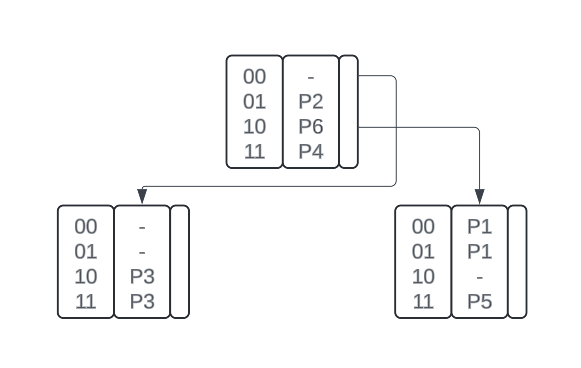
\includegraphics[width=0.7\linewidth]{st_drevo_1.png}
    \caption{Fixed stride številsko drevo s stride velikostjo 2.}
    \label{slika1}
\end{figure}
Prvotno dobimo drevo na sliki \ref*{slika1}. Ker je {\fontfamily{pcr}\selectfont P3} edini naslov, ki se začne z {\fontfamily{pcr}\selectfont 00}, ga lahko prestavimo v prvo tabelo. Tako dobimo drevo na sliki \ref*{slika2}


\begin{figure}[h!]
    \centering
    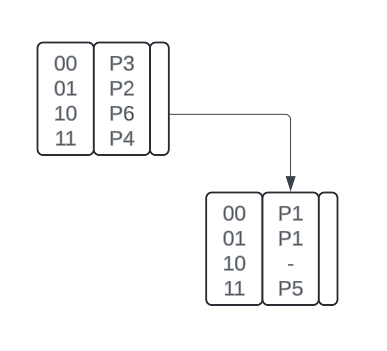
\includegraphics[width=0.5\linewidth]{st_drevo.png}
    \caption{Popravljeno fixed stride številsko drevo s stride velikostjo 2.}
    \label{slika2}
\end{figure}

\pagebreak

\section*{Naloga 3: Kompaktne podatkovne strukture}

\subsection*{BP in LOUDS oblika ordinalnega drevesa}
BP oblika: ((()(()))((()()))) oziroma {\fontfamily{pcr}\selectfont 111011000111010000}, kjer {\fontfamily{pcr}\selectfont 1} predstavlja oklepaj in {\fontfamily{pcr}\selectfont 0} predstavlja zaklepaj.

\noindent
LOUDS oblika: {\fontfamily{pcr}\selectfont 1011011010010110000} oziroma v tabelarični obliki
\begin{table}[htbp]
    \centering
    \begin{tabular}{|c|c|c|c|c|c|c|c|c|c|}
        \hline
        & a & b & c & d & e & f & g & h & i \\
        10 & 110 & 110 & 10 & 0 & 10 & 110 & 0 & 0 & 0 \\
        \hline
    \end{tabular}
\end{table}

\subsection*{BP in LOUDS oblika kardinalnega drevesa}

V kardinalnem drevesu je pomembno ali je otrok levi ali desni, zato liste označujemo z (()()), vozlišča, ki imajo le levega otroka z ($T$()), vozlišča, ki imajo le desnega otroka z (()$T$), kjer je $T$ BP oblika poddrevesa, vozlišča, ki imajo tako levega kot tudi desnega otroka pa predstavimo z ($T_1$ $T_2$), kjer je $T_1$ levo poddrevo, $T_2$ pa desno.

\noindent
BP oblika: (((()())((()())()))(()((()())(()())))) oziroma

\quad \qquad {\fontfamily{pcr}\selectfont 11110100111010010001101110100110100000}.

\noindent
V LOUDS obliki kardinalnega (binarnega) drevesa je vsako vozlišče predstavljeno s tremi biti. Prvi bit je {\fontfamily{pcr}\selectfont 1}, če je lelo poddrevo neprazno, sicer je {\fontfamily{pcr}\selectfont 0}, drugi bit je {\fontfamily{pcr}\selectfont 1}, če je desno poddrevo neprazno, sicer je {\fontfamily{pcr}\selectfont 0}, tretji bit je vedno {\fontfamily{pcr}\selectfont 0} in označuje konec vozlišča.

\noindent
LOUDS oblika: {\fontfamily{pcr}\selectfont 10110110010000100110000000000}
\begin{table}[htbp]
    \centering
    \begin{tabular}{|c|c|c|c|c|c|c|c|c|c|}
        \hline
        & a & b & c & d & e & f & g & h & i \\
        10 & 110 & 110 & 010 & 000 & 100 & 110 & 000 & 000 & 000 \\
        \hline
    \end{tabular}
\end{table}

\subsection*{rmM-drevo}
BP obliko kardinalnega drevesa razdelimo na bloke dolžine $b = 8$.
Najprej izračunamo razliko viškov na začetku in koncu bloka, minimalni višek, maksimalni višek in število maksimalnih viškov vsakega bloka od $s$ do $e$ po naslednjih formulah:
\begin{align*}
    \text{višek (B, i)} &= 2 \text{Rank}_1 \text{(B, i)} - \text{i} \\ 
    \text{e} &= \text{višek (B, e)} - \text{višek (B, s - 1)} \\
    \text{m} &= \min \{ \text{višek (B, p)} - \text{višek (B, s - 1)} | s \leq p \leq e \} \\
    \text{M} &= \max \{ \text{višek (B, p)} - \text{višek (B, s - 1)} | s \leq p \leq e \} \\
\end{align*}
S tem dobimo liste rmM-drevesa. Vsebino vozlišč, ki niso listi izračunamo po naslednjih formulah:
\begin{align*}
    \text{e} &= \text{e}_L + \text{e}_D \\
    \text{m} &= \min \{ \text{m}_L, \text{e}_L + \text{m}_D \} \\
    \text{M} &= \max \{ \text{M}_L, \text{e}_L + \text{M}_D \} \\
    \text{n} &=
    \begin{cases}
        \text{n}_L \quad | \quad \text{m}_L < \text{e}_L + \text{m}_D \\
        \text{n}_D \quad | \quad \text{m}_L > \text{e}_L + \text{m}_D \\
        \text{n}_L + \text{n}_D \quad | \quad \text{m}_L = \text{e}_L + \text{m}_D 
    \end{cases}
    \text{,}
\end{align*}
kjer je e$_L$ višek levega poddrevesa in e$_D$ višek desnega. Ostale oznake so analogne. Tako dobimo naslednje rmM-drevo.

\begin{figure}[h]
    \centering
    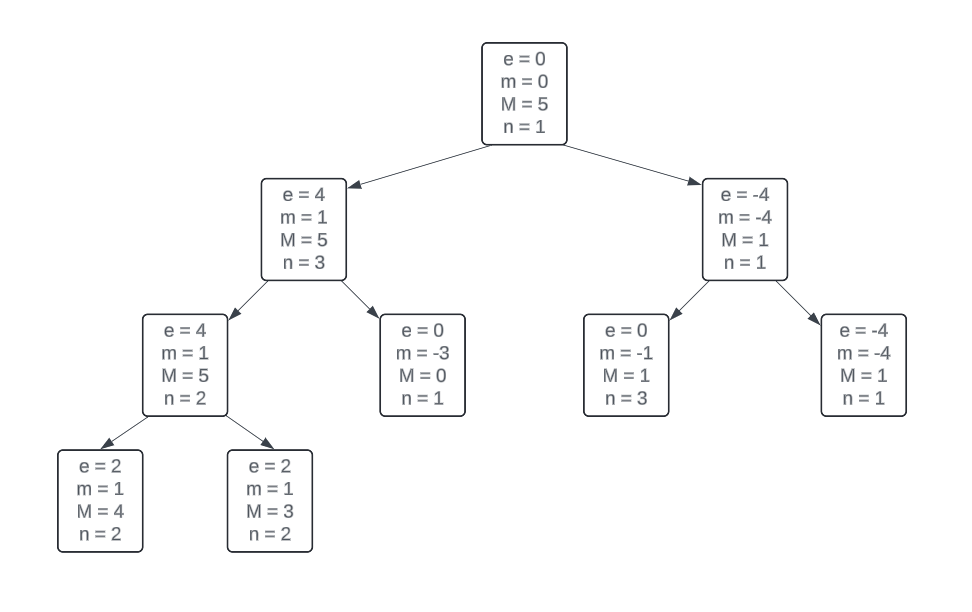
\includegraphics[width=0.9\linewidth]{rmm.png}
    \caption{rmM-drevo z velikostjo blokov $b = 8$.}
\end{figure}

\subsection*{Funkcija {\fontfamily{pcr}\selectfont Izberi (T, i)}}
V tej nalogi zapišemo kodo za iskanje $i$-tega elementa v razširjenem drevesu $T$. Če poznamo velikost levega poddrevesa vsakega vozlišča, je koda naslednja:
\begin{align*}
    &\text{\textbf{definition} Izberi (T, i)} \\
    &\qquad \text{\textbf{if} i $= |$ L $| + 1$ \textbf{then}} \\
    &\qquad \qquad \text{\textbf{return} root(T)}  \\
    &\qquad \text{\textbf{if} i $< |$ L $| +$ 1 \textbf{then}} \\
    &\qquad \qquad \text{\textbf{return} Izberi (L, i)} \\
    &\qquad \text{\textbf{if} i $> |$ L $| +$ 1 \textbf{then}} \\
    &\qquad \qquad \text{\textbf{return} Izberi (R, i $- |$ L $| -$ 1)}   
\end{align*}
Velikost levega poddrevesa primerjamo z danim $i$. V kolikor je $i = |L| + 1$ je $i$-to vozlišče kar koren drevesa $T$.
Če je $i < |L| + 1$ iščemo $i$-to vozlišče levega poddrevesa, sicer pa $i - |L| - 1$-vo vozlišče desnega poddrevesa.

\end{document}